% Chapter 1

\chapter{Hardware Architecture for Inter-Prediction} % Write in your own chapter title
\label{Chapter4}
\lhead{Chapter 4. \emph{Thesis Structure}} % Write in your own chapter title to set the page header

There are many new technologies such as intra prediction, in loop deblocking filter, context based arithmetic coding introduced in the latest H.264/AVC standard. Among all of these amazing technologies, \textbf{Variable Block Size Motion Estimation (VBSME)} is one of the powerful techniques. In comparison with the previous Fixed Block Size Motion Estimation (FBSME), VBSME divides one MB into smaller blocks to fit the different motion directions. In this way, the coding performance is proved.

We designed a parallel \textbf{265 PE VBS ME Hardware Architecture}. This hardware is implemented in System Verilog. First of all, the pixels in the current MB are stored in a Block Ram \textbf{(c$\_$BRAM)}. The pixels of the search window are also stored in a block RAM \textbf{(s$\_$BRAM)}. The architecture is shown in the figure \ref{fig:256pevbsme}

\begin{figure}[htbp]
	\centering
	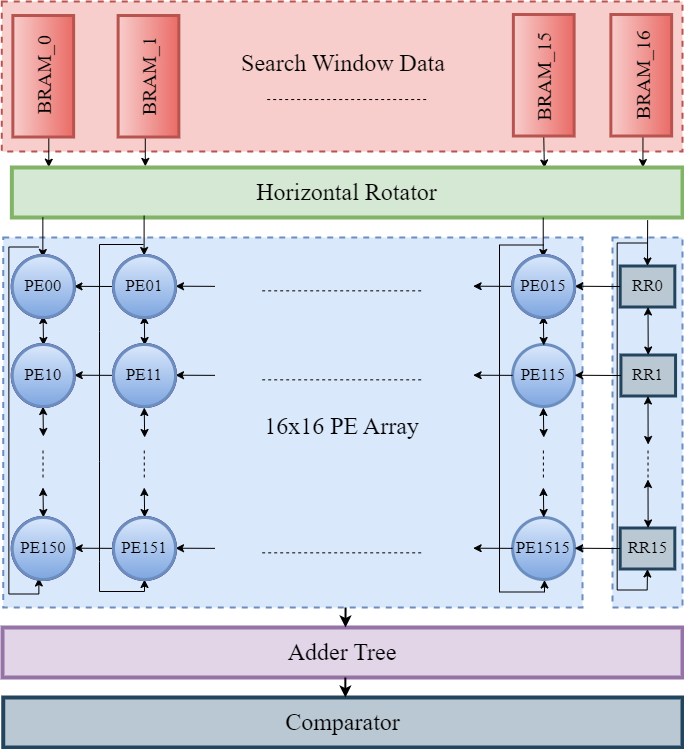
\includegraphics[width = 4in]{./Figures/256pevbsme.png}
	\rule{35em}{0.5pt}
	\caption{265 PE VBS ME Hardware Architecture}
	\label{fig:256pevbsme}
\end{figure}

In this design, a \textbf{2-D systolic PE array} is used. (what is 2d systolic pe array explain). There are \textbf{16x16 = 256 PEs} ( 16 rows and 16 columns) and all of them are  made capable of shifting data down, up and left. For a \textbf{16x16 MB}, a Motion Vector MV is found in one cycle in a search range of \textbf{[-16, 15]} pixels.



